\documentclass[accentcolor=tud2c,usenames,dvipsnames,colorbacktitle,inverttitle,landscape,german,presentation,t]{tudbeamer}
\usepackage[english]{babel}
\usepackage{amsmath}
\usepackage{amssymb}
\usepackage{color}
\usepackage{physics}
\usepackage{graphicx}
\usepackage{braket}
\usepackage[utf8]{inputenc}

\begin{document}
  \setbeamerfont{footline}{size=\fontsize{1}{1}\selectfont}

  \title{QCD critical point searches at STAR}
  \subtitle{\small{Matthias Heinz}}
  \author{Matthias Heinz}
  \institute[Institut f\"ur Kernphysik, TU Darmstadt]{Institut f\"ur Kernphysik, TU Darmstadt}
  \date{July 10, 2019}

  \setbeamertemplate{section in toc}[ball unnumbered]
  \setbeamertemplate{subsection in toc}[ball unnumbered]

  \nocite{*}

  \begin{titleframe}
    \begin{center}
      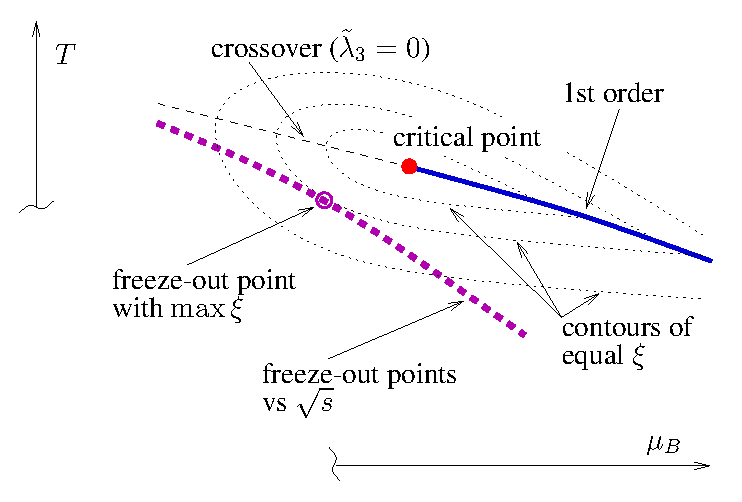
\includegraphics[width=0.75\textwidth]{figures/05/critical_point_illustration}
      \\\footnotesize{Stephanov 2009}
    \end{center}
  \end{titleframe}

  \section{Introduction}

  \begin{frame}
    \frametitle{The RHIC beam energy scan}
    \begin{columns}[c]
      \begin{column}{0.4\textwidth}
        \begin{itemize}
          \item Quark-gluon plasma
          \item Hadron gas
          \item First-order phase transition and critical point
        \end{itemize}
      \end{column}
      \begin{column}{0.6\textwidth}
        \begin{center}
          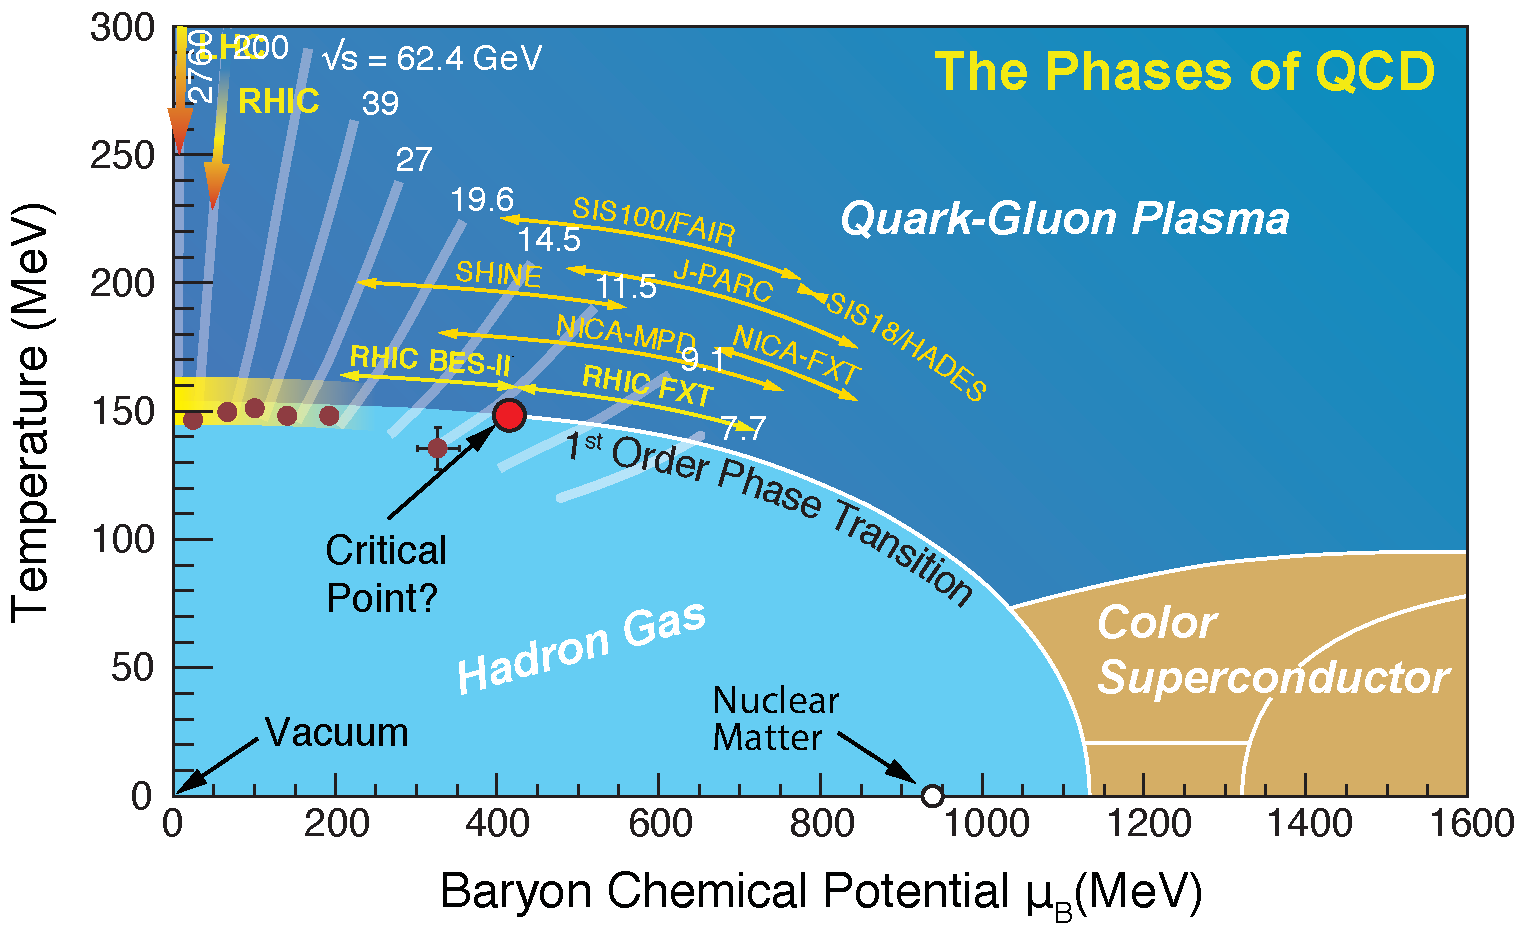
\includegraphics[width=\textwidth]{figures/02/PhaseDiagram}
          \\ \footnotesize{Caines 2017}
        \end{center}
      \end{column}
    \end{columns}
  \end{frame}

  \section{Experimental signatures}

  \begin{frame}
    \frametitle{Critical point physics \\ \small{\textit{Stephanov,
    Rajagopal}}}
    \begin{itemize}
      \item Critical mode $\sigma$ which develops infinite correlation length
        $\xi$ near critical point
      \item Treat $\sigma$ as a classical field
      \item Note that for the zero momentum mode $\sigma_0 = \int d^3x
        \sigma(x)/V$, there are cumulants:
    \end{itemize}
    \begin{equation*}
      \kappa_2 = \expectationvalue{\sigma_{0}^{2}} = \frac{T}{V} \xi^2
    \end{equation*}
    \begin{equation*}
      \kappa_3 = \expectationvalue{\sigma_{0}^{3}} \sim \frac{T}{V} \xi^6
    \end{equation*}
    \begin{equation*}
      \kappa_4 = \expectationvalue{\sigma_{0}^{4}}_c \sim \frac{T}{V} \xi^8
    \end{equation*}
    \begin{itemize}
      \item Higher-order cumulants are especially sensitive to the increase in
        the correlation length
      \end{itemize}
  \end{frame}

  \begin{frame}
    \frametitle{Critical point observables}
    \begin{itemize}
      \item Can adopt similar approach to distributions of conserved quantities
        in experiment
      \begin{itemize}
        \item Net baryon number $B$
        \item Net charge $Q$
        \item Net strangeness $S$
      \end{itemize}
      \item Connect to theory via susceptibility $\chi$
    \end{itemize}
    \begin{equation*}
      \chi_{B}^{(n)} = \frac{1}{V T^3} C_{n,B}
    \end{equation*}
    \begin{itemize}
      \item Measurements of event-by-event fluctuations of conserved quantities allow
        us to observe critical point
    \end{itemize}
  \end{frame}

  \begin{frame}
    \frametitle{Overall approach}
    \begin{itemize}
      \item Lower $\sqrt{s_{NN}}$ probes larger $\mu_B$
      \item At beam energy scan energies, collision centrality affects $\mu_B$
        as well
    \end{itemize}
    \begin{center}
      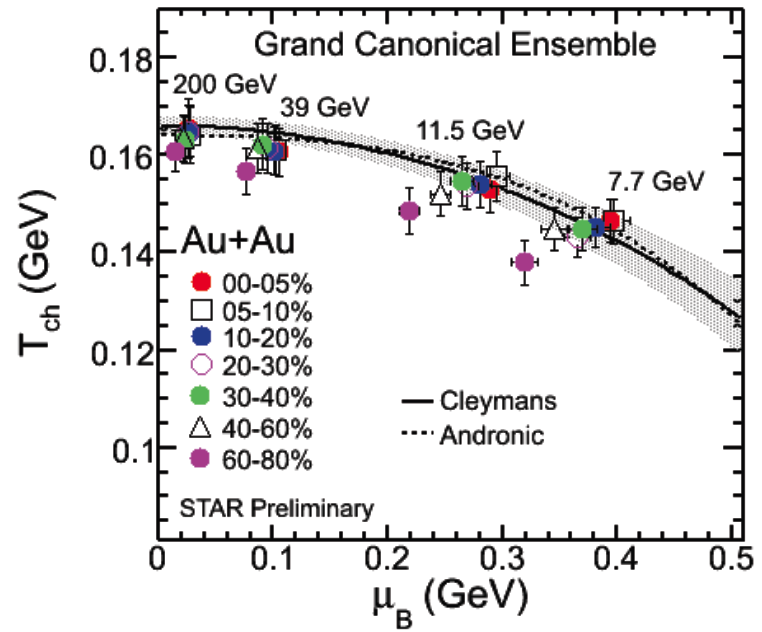
\includegraphics[width=0.42\textwidth]{figures/05/freezeout_diagram}
      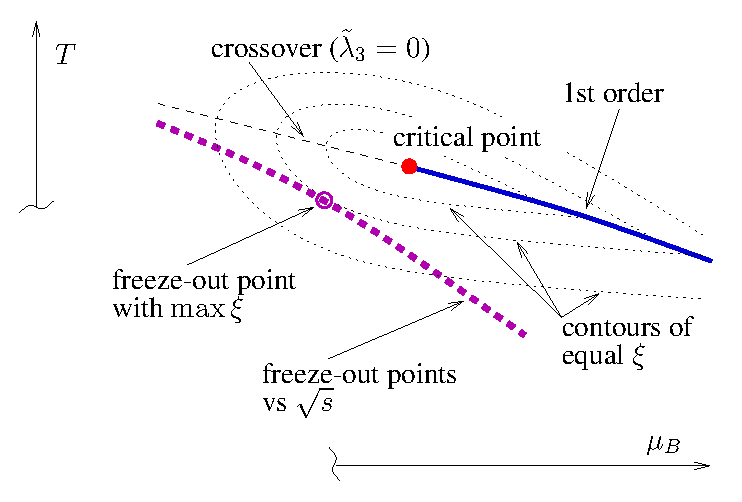
\includegraphics[width=0.54\textwidth]{figures/05/critical_point_illustration}
      \\\footnotesize{STAR (Schmah et al.) 2013~~~~~~~~~~~~~~~~~~~~~~~~~~~~~~~~~~~~~Stephanov 2009}
    \end{center}
  \end{frame}


  \section{STAR detector and analysis}

  \begin{frame}
    \frametitle{The STAR detector}
    \begin{overprint}
      \onslide<1>\begin{center}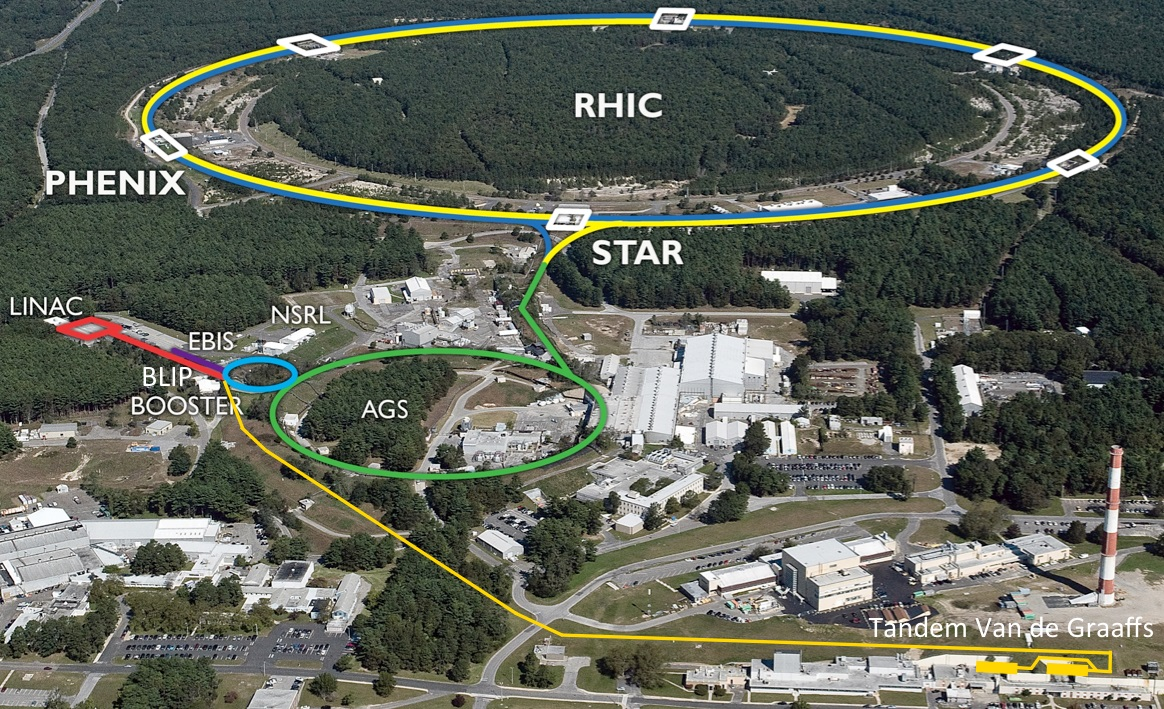
\includegraphics[width=0.8\textwidth]{figures/06/RHIC}\\\footnotesize{BNL 2019}\end{center}
      \onslide<2->\begin{center}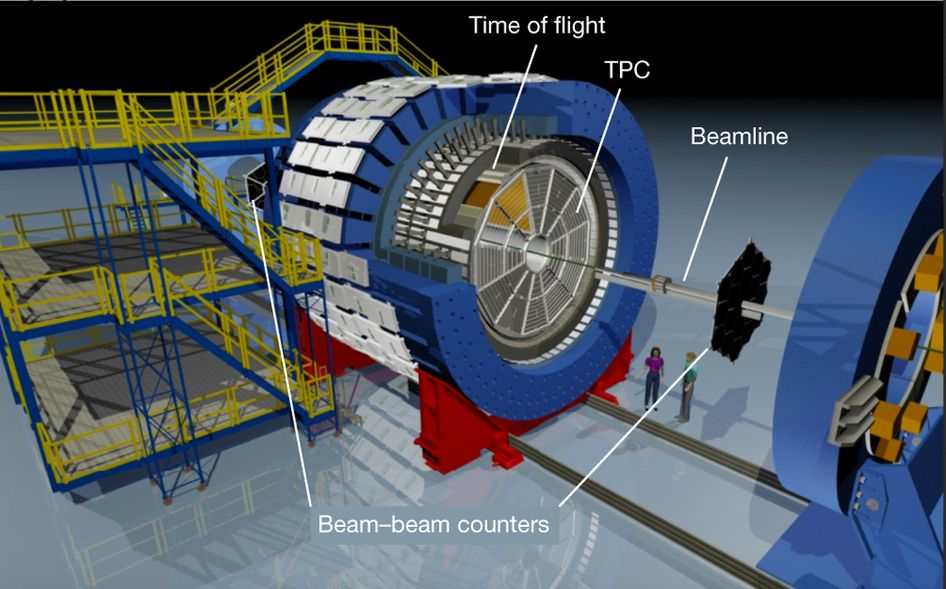
\includegraphics[width=0.75\textwidth]{figures/06/star_detector}\\\footnotesize{STAR (Adamcyzk et al.) 2017}\end{center}
    \end{overprint}
  \end{frame}

  \begin{frame}
    \frametitle{Net proton number measurements}
    \begin{itemize}
      \item Consider net proton number $\Delta N_p$ as proxy for net baryon
        number
      \item Can also consider as proxy for net charge number
    \end{itemize}
    \begin{equation*}
      \Delta N_p = N_p - N_{\bar{p}}
    \end{equation*}
    \begin{itemize}
      \item Au+Au collisions
      \item Center-of-mass energies: 7.7, 11.5, 19.6, 27, 39, 62.4, and 200 GeV
      \item Transverse momentum range: $0.4 < p_T < 2$ GeV/c
      \item Pseudorapidity acceptance: $|\eta| < 1.0$
    \end{itemize}
  \end{frame}

  \begin{frame}
    \frametitle{Centrality bin width correction}
    \begin{itemize}
      \item Minimum centrality bin size is single value for particle
        multiplicity
      \item Typically work in terms of ranges, like 0-5\%
      \item Need to correctly assemble cumulant value within a larger
        centrality bin
    \end{itemize}
    \begin{equation*}
      C_n = \frac{\sum_{r=N_1}^{N_2} n_r C_{n}^{r}}{\sum_{r=N_1}^{N_2} n_r} =
      \sum_{r=N_1}^{N_2} \omega_r C_{n}^{r}
    \end{equation*}
    \begin{itemize}
      \item Corrected cumulants can be used to compute cumulant ratios
      \item Propagation of statistical errors is straightforward
      \item Question: Why not apply the same treatment to cumulant ratios?
    \end{itemize}
    \begin{equation*}
      \frac{\sum_{r=N_1}^{N_2} \omega_r C_{n}^{r}}{\sum_{r=N_1}^{N_2} \omega_r
      C_{m}^{r}} \neq
      \sum_{r=N_1}^{N_2} \omega_r \frac{C_{n}^{r}}{C_{m}^{r}}
    \end{equation*}
  \end{frame}

  \begin{frame}
    \frametitle{Determining centrality}
    \begin{itemize}
      \item Care needs to be taken when determining centrality
      \item In general, more particles used in centrality allows for better
        resolution
      \item However, we need to avoid autocorrelation effects by determining
        centrality with the same particles used later in the analysis
      \item Introduce new centrality definition:
      \begin{itemize}
        \item For net-proton analyses, determine centrality with charged kaon
          and pion multiplicities in $|\eta| < 1$
        \item For net-charge analyses (not discussed here), use particles in
          $0.5 < |\eta| < 1$ and do analysis with particles in $|\eta| < 0.5$
      \end{itemize}
    \end{itemize}
  \end{frame}

  \begin{frame}
    \frametitle{Efficiency correction and statistical error estimation}
    \begin{columns}[c]
      \begin{column}{0.5\textwidth}
        \begin{center}
          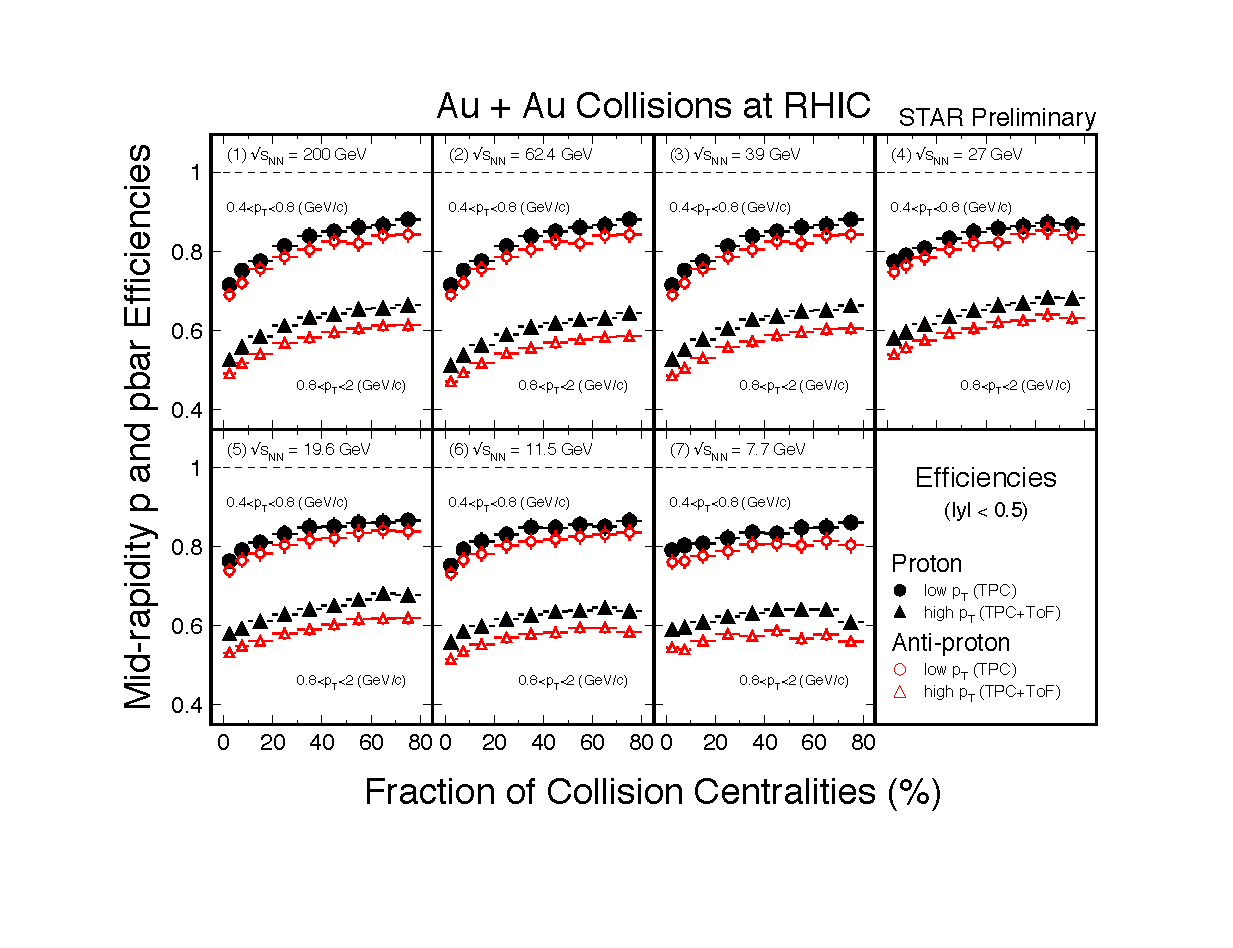
\includegraphics[width=1.0\textwidth]{figures/10/peff_BES}
          \\\footnotesize{STAR (Luo et al.) 2015}
        \end{center}
      \end{column}
      \begin{column}{0.5\textwidth}
        \begin{itemize}
          \item Need to account for detector efficiency
          \item Particle identification is handled differently
            for low and high $p_T$
          \begin{itemize}
            \item For $0.4 < p_T < 0.8$ GeV/c, only the TPC is used
            \item For $0.8 < p_T < 2.0$ GeV/c, both TOF and TPC are used
          \end{itemize}
          \item Estimate statistical error along with efficiency correction
            (Delta theorem)
          \item Should take place just before doing centrality bin width
            correction
        \end{itemize}
      \end{column}
    \end{columns}
  \end{frame}


  \section{Results}

  \begin{frame}
    \frametitle{Observed cumulants up to fourth order}
    \begin{center}
      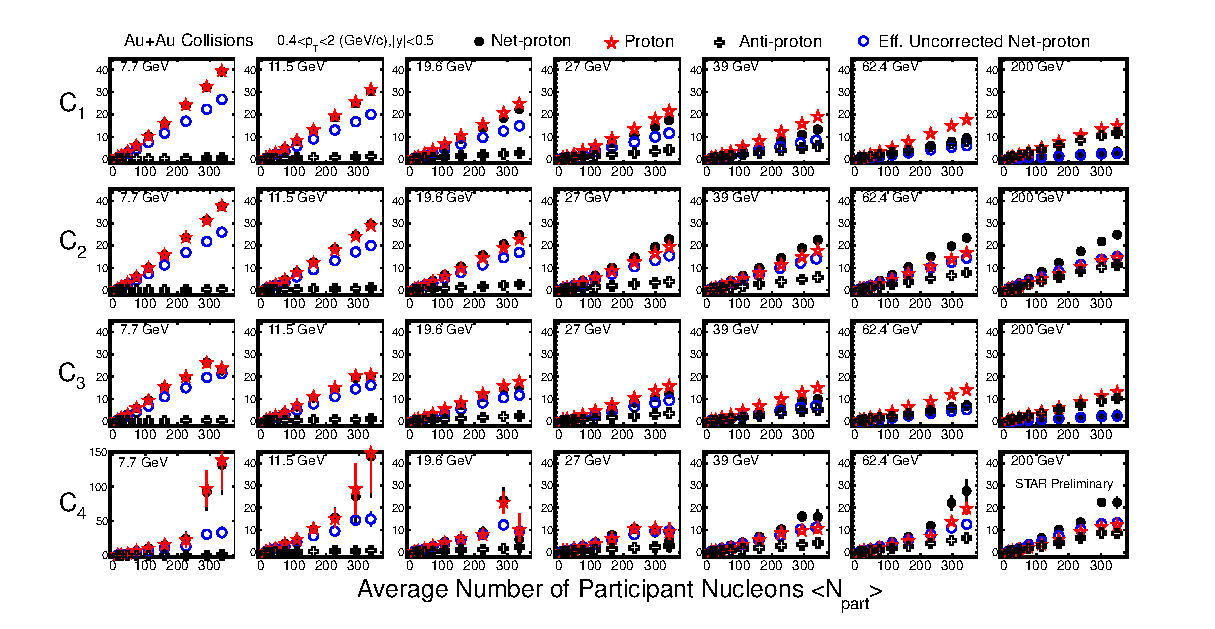
\includegraphics[width=0.9\textwidth]{figures/11/Cumulants}
      \\\footnotesize{STAR (Luo et al.) 2015}
    \end{center}
  \end{frame}

  \begin{frame}
    \frametitle{Cumulant ratios}
    \begin{columns}[c]
      \begin{column}{0.6\textwidth}
      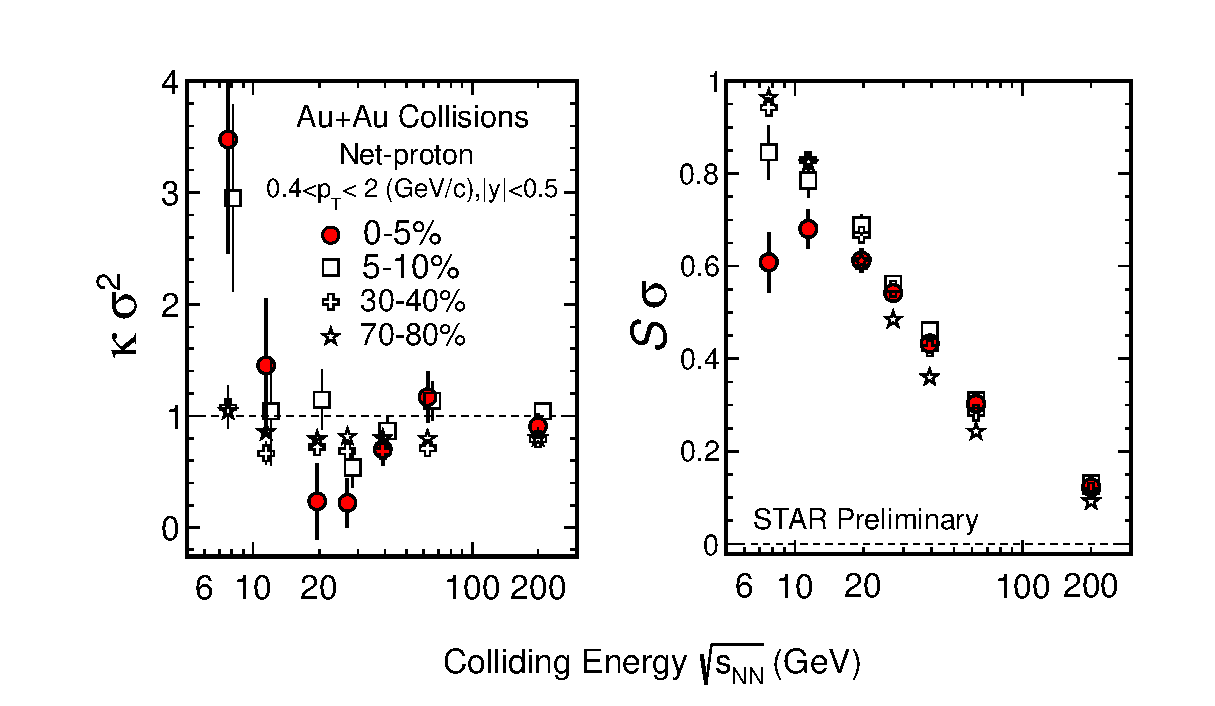
\includegraphics[width=\textwidth]{figures/12/Energy_KV_SD}
      \begin{center}
        \footnotesize{STAR (Luo et al.) 2015}
      \end{center}
      \end{column}
      \begin{column}{0.4\textwidth}
        \begin{equation*}
          \kappa \sigma^2 = C_4 / C_2
        \end{equation*}
        \begin{equation*}
          S \sigma = C_3 / C_2
        \end{equation*}
        \begin{itemize}
          \item Form ratios of cumulants to cancel volume and temperature
            dependence
          \item $S$ is skewness
          \item $\kappa$ is kurtosis
        \end{itemize}
      \end{column}
    \end{columns}
  \end{frame}

  \begin{frame}
    \frametitle{Skellam distributions}
    \begin{center}
      \vskip-1em
      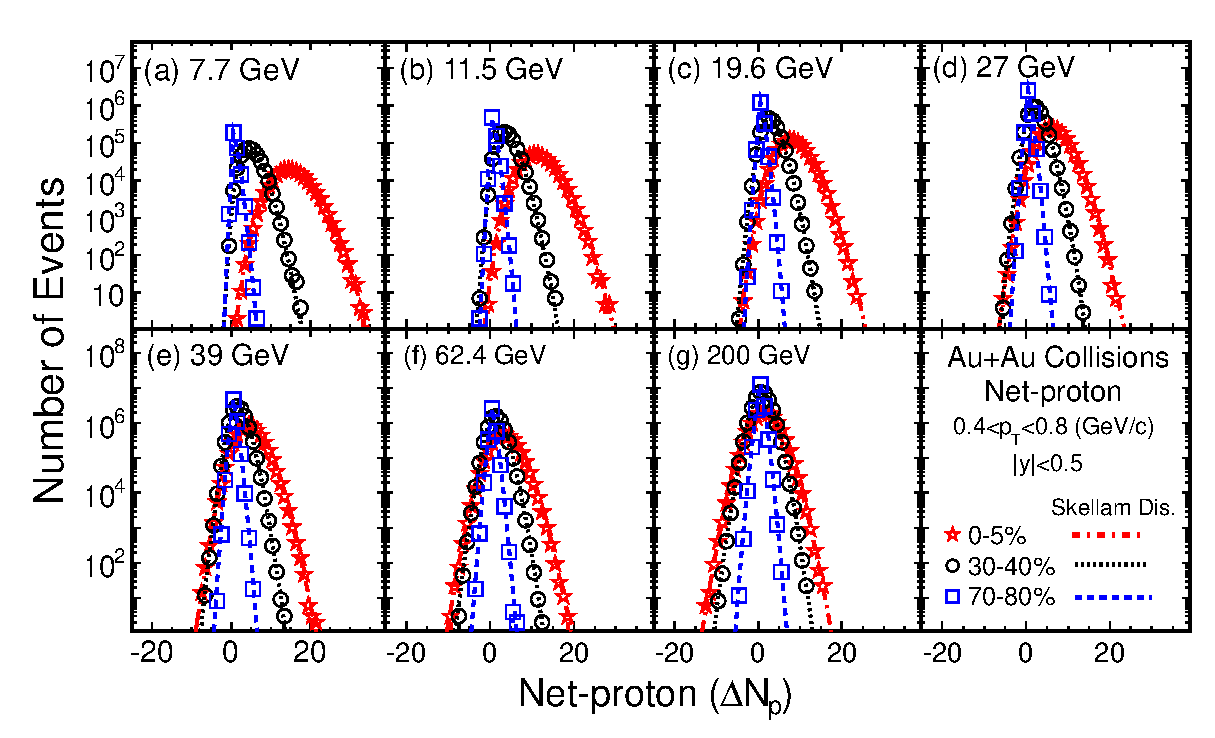
\includegraphics[width=0.6\textwidth]{figures/13/Fig1}
      \\\footnotesize{STAR (Adamcyzk et al.) 2014}
    \end{center}
    \begin{itemize}
      \item Assume protons and anti-protons are distributed as if sampled from
        independent Poisson distributions
      \item Represents thermal statistical fluctuations of net-proton number
    \end{itemize}
  \end{frame}

  \begin{frame}
    \frametitle{$\kappa \sigma^2$ and $S \sigma / \text{Skellam}$}
    \begin{center}
      \vskip-2em
      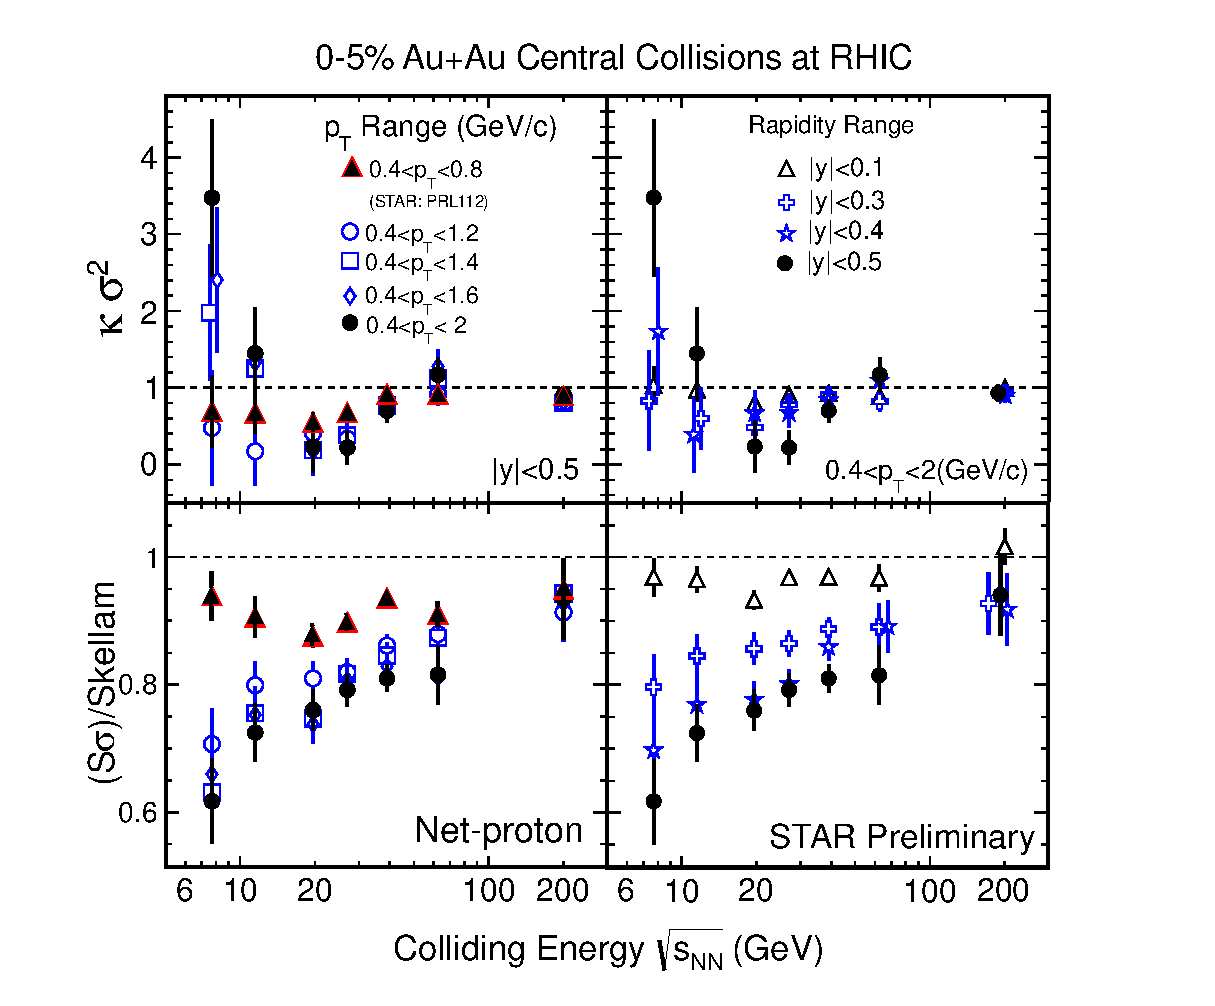
\includegraphics[width=0.65\textwidth]{figures/14/PT_Y_Energy}
      \\\footnotesize{STAR (Luo et al.) 2015}
    \end{center}
  \end{frame}

  \section{Looking forward}

  \begin{frame}
    \frametitle{Beam energy scan II}
    \begin{columns}[c]
      \begin{column}{0.6\textwidth}
        \begin{itemize}
          \item Run at $\sqrt{s_{NN}} = 9.1$ GeV in addition to BES-I energies
          \item Energies below 7.7 GeV via fixed-target program
          \item Detector upgrades:
          \begin{itemize}
            \item iTPC: inner time projection chamber with wider acceptance
              $|\eta| < 1.5$ and higher resolution
            \item EPD: event plane detector to better determine event plane and
              offer improved centrality determination
          \end{itemize}
        \end{itemize}
      \end{column}
      \begin{column}{0.4\textwidth}
        \begin{center}
          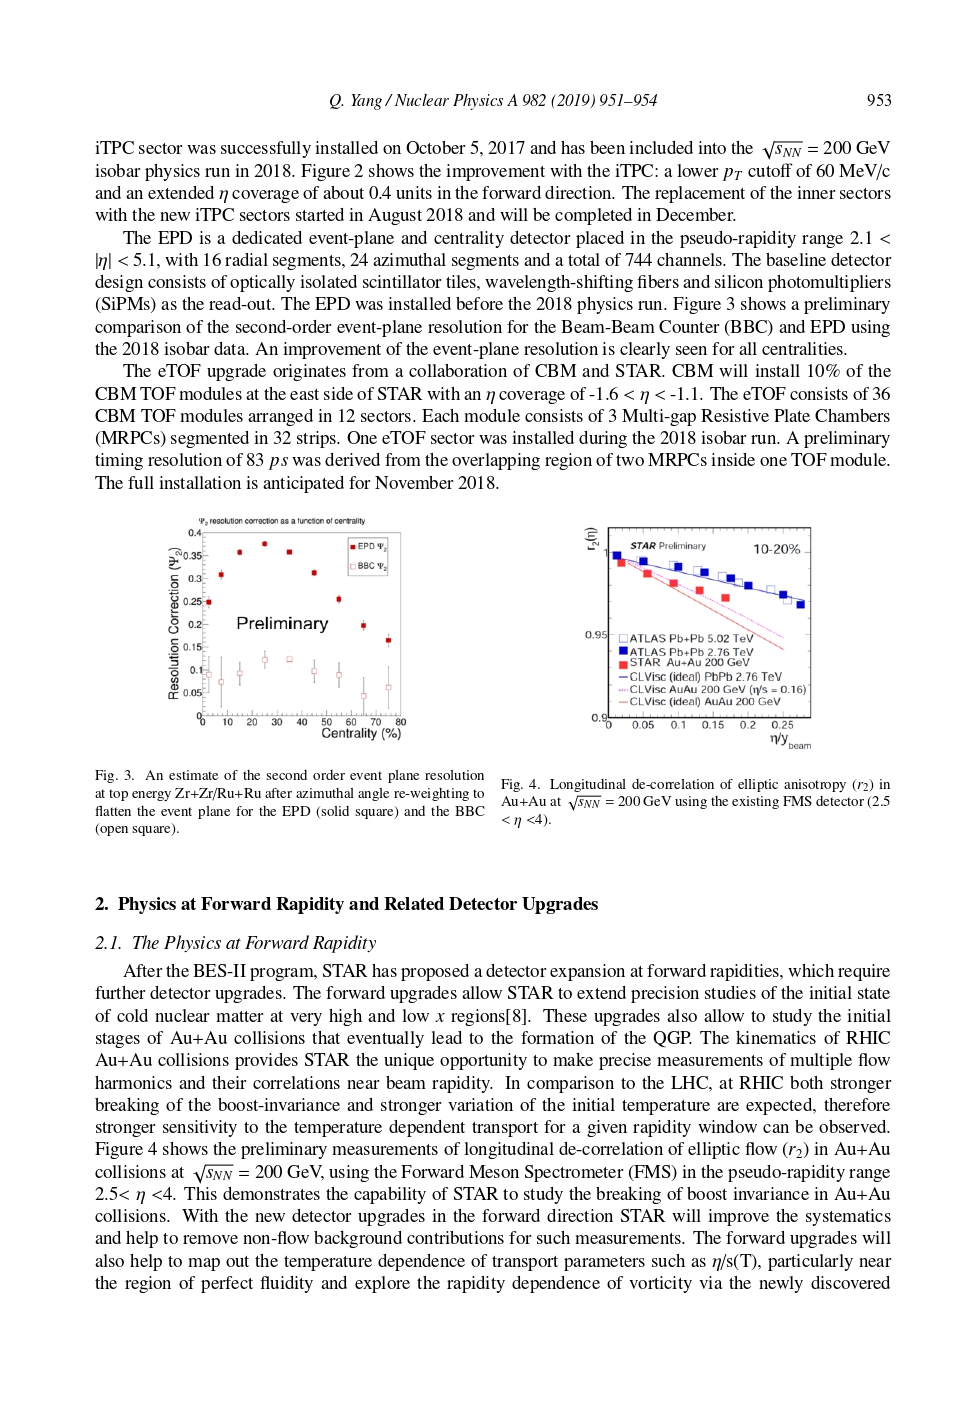
\includegraphics[trim={2.4cm 11.4cm 8.5cm 8.5cm},clip,width=\textwidth]{figures/15/epd}
          \\\footnotesize{STAR (Yang et al.) 2019}
        \end{center}
      \end{column}
    \end{columns}
  \end{frame}

  \section{Summary}

  \begin{frame}
    \frametitle{Summary}
    \begin{columns}[c]
      \begin{column}{0.6\textwidth}
        \begin{itemize}
          \item Key ideas:
          \begin{itemize}
            \item Look to higher cumulants of distributions of conserved
              quantities
            \item Use ratios to cancel dependence on quantities other than
              $\xi$
            \item Look for non-monotonic behavior in ratios
          \end{itemize}
          \item Results seem suggestive, but not conclusive
          \item Would like theoretical predictions for susceptibility ratios
          \item Need better statistics $\rightarrow$ BES-II
        \end{itemize}
      \end{column}
      \begin{column}{0.4\textwidth}
        \begin{center}
          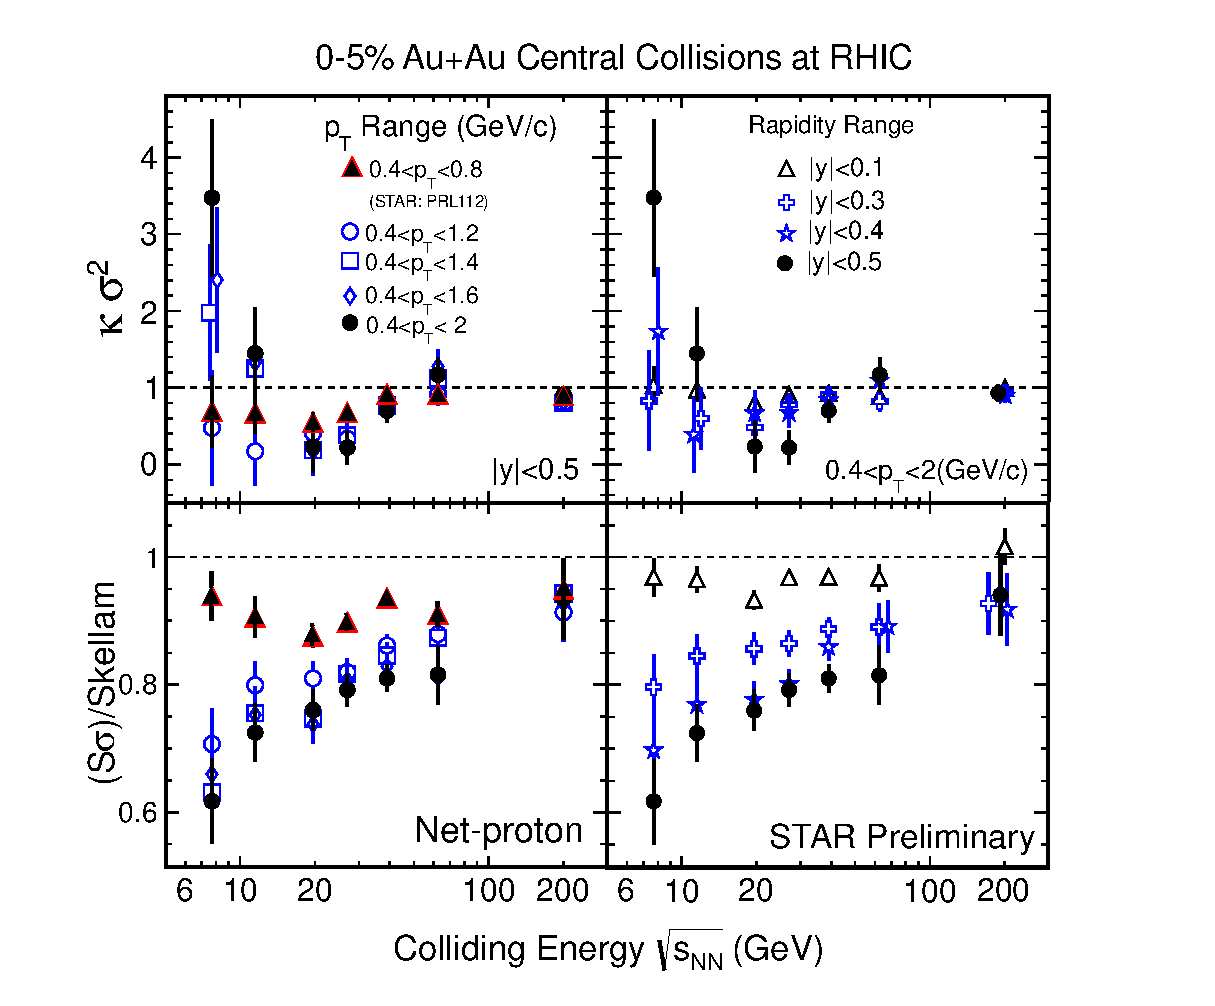
\includegraphics[width=\textwidth]{figures/14/PT_Y_Energy}
          \\\footnotesize{STAR (Luo et al.) 2015}
        \end{center}
      \end{column}
    \end{columns}
  \end{frame}


  \begin{frame}[allowframebreaks]
    \frametitle{References}
    \bibliographystyle{apalike}
    \bibliography{bibfile}
  \end{frame}

\end{document}
